\documentclass[a4paper]{article}

\usepackage[pdftex,
  hidelinks,
  pdfauthor={Dexter Chua},
  pdfsubject={Cambridge Maths Notes: Part IB - Electromagnetism},
  pdftitle={Part IB - Electromagnetism},
pdfkeywords={Cambridge Mathematics Maths Math IB Lent Electromagnetism}]{hyperref}

\title{Part IB - Electromagnetism}
\author{Lectured by David Tong}
\date{Lent 2015}

% Imports
\ifx \nextra \undefined
  \usepackage[pdftex,
    hidelinks,
    pdfauthor={Dexter Chua},
    pdfsubject={Cambridge Maths Notes: Part \npart\ - \ncourse},
    pdftitle={Part \npart\ - \ncourse},
  pdfkeywords={Cambridge Mathematics Maths Math \npart\ \nterm\ \nyear\ \ncourse}]{hyperref}
  \title{Part \npart\ - \ncourse}
\else
  \usepackage[pdftex,
    hidelinks,
    pdfauthor={Dexter Chua},
    pdfsubject={Cambridge Maths Notes: Part \npart\ - \ncourse\ (\nextra)},
    pdftitle={Part \npart\ - \ncourse\ (\nextra)},
  pdfkeywords={Cambridge Mathematics Maths Math \npart\ \nterm\ \nyear\ \ncourse\ \nextra}]{hyperref}

  \title{Part \npart\ - \ncourse \\ {\Large \nextra}}
\fi

\author{Lectured by \nlecturer \\\small Notes taken by Dexter Chua}
\date{\nterm\ \nyear}

\usepackage{alltt}
\usepackage{amsfonts}
\usepackage{amsmath}
\usepackage{amssymb}
\usepackage{amsthm}
\usepackage{booktabs}
\usepackage{caption}
\usepackage{enumitem}
\usepackage{fancyhdr}
\usepackage{graphicx}
\usepackage{mathtools}
\usepackage{microtype}
\usepackage{multirow}
\usepackage{pdflscape}
\usepackage{pgfplots}
\usepackage{siunitx}
\usepackage{tabularx}
\usepackage{tikz}
\usepackage{tkz-euclide}
\usepackage[normalem]{ulem}
\usepackage[all]{xy}

\pgfplotsset{compat=1.12}

\pagestyle{fancyplain}
\lhead{\emph{\nouppercase{\leftmark}}}
\ifx \nextra \undefined
  \rhead{
    \ifnum\thepage=1
    \else
      \npart\ \ncourse
    \fi}
\else
  \rhead{
    \ifnum\thepage=1
    \else
      \npart\ \ncourse\ (\nextra)
    \fi}
\fi
\usetikzlibrary{arrows}
\usetikzlibrary{decorations.markings}
\usetikzlibrary{decorations.pathmorphing}
\usetikzlibrary{positioning}
\usetikzlibrary{fadings}
\usetikzlibrary{intersections}
\usetikzlibrary{cd}

\newcommand*{\Cdot}{\raisebox{-0.25ex}{\scalebox{1.5}{$\cdot$}}}
\newcommand {\pd}[2][ ]{
  \ifx #1 { }
    \frac{\partial}{\partial #2}
  \else
    \frac{\partial^{#1}}{\partial #2^{#1}}
  \fi
}

% Theorems
\theoremstyle{definition}
\newtheorem*{aim}{Aim}
\newtheorem*{axiom}{Axiom}
\newtheorem*{claim}{Claim}
\newtheorem*{cor}{Corollary}
\newtheorem*{defi}{Definition}
\newtheorem*{eg}{Example}
\newtheorem*{fact}{Fact}
\newtheorem*{law}{Law}
\newtheorem*{lemma}{Lemma}
\newtheorem*{notation}{Notation}
\newtheorem*{prop}{Proposition}
\newtheorem*{thm}{Theorem}

\renewcommand{\labelitemi}{--}
\renewcommand{\labelitemii}{$\circ$}
\renewcommand{\labelenumi}{(\roman{*})}

\let\stdsection\section
\renewcommand\section{\newpage\stdsection}

% Strike through
\def\st{\bgroup \ULdepth=-.55ex \ULset}

% Maths symbols
\newcommand{\bra}{\langle}
\newcommand{\ket}{\rangle}

\newcommand{\N}{\mathbb{N}}
\newcommand{\Z}{\mathbb{Z}}
\newcommand{\Q}{\mathbb{Q}}
\renewcommand{\H}{\mathbb{H}}
\newcommand{\R}{\mathbb{R}}
\newcommand{\C}{\mathbb{C}}
\newcommand{\Prob}{\mathbb{P}}
\renewcommand{\P}{\mathbb{P}}
\newcommand{\E}{\mathbb{E}}
\newcommand{\F}{\mathbb{F}}
\newcommand{\cU}{\mathcal{U}}
\newcommand{\RP}{\mathbb{RP}}
\newcommand{\CP}{\mathbb{CP}}

\newcommand{\ph}{\,\cdot\,}

\DeclareMathOperator{\sech}{sech}
\DeclareMathOperator{\cosech}{cosech}
\DeclareMathOperator{\cosec}{cosec}

\DeclareMathOperator{\covol}{covol}
\DeclareMathOperator{\vol}{vol}

\let\Im\relax
\let\Re\relax
\DeclareMathOperator{\Im}{Im}
\DeclareMathOperator{\Re}{Re}
\DeclareMathOperator{\im}{im}
\DeclareMathOperator{\image}{image}
\DeclareMathOperator{\Ann}{Ann}

\DeclareMathOperator*{\res}{res}
\DeclareMathOperator{\Res}{Res}
\DeclareMathOperator{\Ind}{Ind}

\DeclareMathOperator{\tr}{tr}
\DeclareMathOperator{\diag}{diag}
\DeclareMathOperator{\rank}{rank}
\DeclareMathOperator{\card}{card}
\DeclareMathOperator{\spn}{span}
\DeclareMathOperator{\adj}{adj}

\DeclareMathOperator{\erf}{erf}
\DeclareMathOperator{\erfc}{erfc}

\DeclareMathOperator{\ord}{ord}
\DeclareMathOperator{\Sym}{Sym}

\DeclareMathOperator{\sgn}{sgn}
\DeclareMathOperator{\orb}{orb}
\DeclareMathOperator{\stab}{stab}
\DeclareMathOperator{\ccl}{ccl}

\DeclareMathOperator{\lcm}{lcm}
\DeclareMathOperator{\hcf}{hcf}

\DeclareMathOperator{\Int}{Int}
\DeclareMathOperator{\id}{id}

\DeclareMathOperator{\betaD}{beta}
\DeclareMathOperator{\gammaD}{gamma}
\DeclareMathOperator{\Poisson}{Poisson}
\DeclareMathOperator{\binomial}{binomial}
\DeclareMathOperator{\multinomial}{multinomial}
\DeclareMathOperator{\Bernoulli}{Bernoulli}
\DeclareMathOperator{\like}{like}

\DeclareMathOperator{\var}{var}
\DeclareMathOperator{\cov}{cov}
\DeclareMathOperator{\bias}{bias}
\DeclareMathOperator{\mse}{mse}
\DeclareMathOperator{\corr}{corr}

\DeclareMathOperator{\otp}{otp}
\DeclareMathOperator{\dom}{dom}

\DeclareMathOperator{\Root}{Root}
\DeclareMathOperator{\supp}{supp}
\DeclareMathOperator{\rel}{rel}
\DeclareMathOperator{\Hom}{Hom}
\DeclareMathOperator{\Aut}{Aut}
\DeclareMathOperator{\Gal}{Gal}
\DeclareMathOperator{\Mat}{Mat}
\DeclareMathOperator{\End}{End}
\DeclareMathOperator{\Char}{char}
\DeclareMathOperator{\ev}{ev}
\DeclareMathOperator{\St}{St}
\DeclareMathOperator{\Lk}{Lk}
\DeclareMathOperator{\disc}{disc}
\DeclareMathOperator{\Isom}{Isom}
\DeclareMathOperator{\length}{length}
\DeclareMathOperator{\energy}{energy}
\DeclareMathOperator{\area}{area}
\DeclareMathOperator{\Syl}{Syl}
\DeclareMathOperator{\cl}{cl}
\DeclareMathOperator{\fix}{fix}

\newcommand{\GL}{\mathrm{GL}}
\newcommand{\SL}{\mathrm{SL}}
\newcommand{\PGL}{\mathrm{PGL}}
\newcommand{\PSL}{\mathrm{PSL}}
\newcommand{\PSU}{\mathrm{PSU}}
\newcommand{\Or}{\mathrm{O}}
\newcommand{\SO}{\mathrm{SO}}
\newcommand{\U}{\mathrm{U}}
\newcommand{\SU}{\mathrm{SU}}

\renewcommand{\d}{\mathrm{d}}
\newcommand{\D}{\mathrm{D}}

\tikzset{->/.style = {decoration={markings,
                                  mark=at position 1 with {\arrow[scale=2]{latex'}}},
                      postaction={decorate}}}
\tikzset{<-/.style = {decoration={markings,
                                  mark=at position 0 with {\arrowreversed[scale=2]{latex'}}},
                      postaction={decorate}}}
\tikzset{<->/.style = {decoration={markings,
                                   mark=at position 0 with {\arrowreversed[scale=2]{latex'}},
                                   mark=at position 1 with {\arrow[scale=2]{latex'}}},
                       postaction={decorate}}}
\tikzset{->-/.style = {decoration={markings,
                                   mark=at position #1 with {\arrow[scale=2]{latex'}}},
                       postaction={decorate}}}
\tikzset{-<-/.style = {decoration={markings,
                                   mark=at position #1 with {\arrowreversed[scale=2]{latex'}}},
                       postaction={decorate}}}

\tikzset{circ/.style = {fill, circle, inner sep = 0, minimum size = 3}}
\tikzset{mstate/.style={circle, draw, blue, text=black, minimum width=0.7cm}}

\definecolor{mblue}{rgb}{0.2, 0.3, 0.8}
\definecolor{morange}{rgb}{1, 0.5, 0}
\definecolor{mgreen}{rgb}{0.1, 0.4, 0.2}
\definecolor{mred}{rgb}{0.5, 0, 0}

\def\drawcirculararc(#1,#2)(#3,#4)(#5,#6){%
    \pgfmathsetmacro\cA{(#1*#1+#2*#2-#3*#3-#4*#4)/2}%
    \pgfmathsetmacro\cB{(#1*#1+#2*#2-#5*#5-#6*#6)/2}%
    \pgfmathsetmacro\cy{(\cB*(#1-#3)-\cA*(#1-#5))/%
                        ((#2-#6)*(#1-#3)-(#2-#4)*(#1-#5))}%
    \pgfmathsetmacro\cx{(\cA-\cy*(#2-#4))/(#1-#3)}%
    \pgfmathsetmacro\cr{sqrt((#1-\cx)*(#1-\cx)+(#2-\cy)*(#2-\cy))}%
    \pgfmathsetmacro\cA{atan2(#2-\cy,#1-\cx)}%
    \pgfmathsetmacro\cB{atan2(#6-\cy,#5-\cx)}%
    \pgfmathparse{\cB<\cA}%
    \ifnum\pgfmathresult=1
        \pgfmathsetmacro\cB{\cB+360}%
    \fi
    \draw (#1,#2) arc (\cA:\cB:\cr);%
}
\newcommand\getCoord[3]{\newdimen{#1}\newdimen{#2}\pgfextractx{#1}{\pgfpointanchor{#3}{center}}\pgfextracty{#2}{\pgfpointanchor{#3}{center}}}

\def\Xint#1{\mathchoice
   {\XXint\displaystyle\textstyle{#1}}%
   {\XXint\textstyle\scriptstyle{#1}}%
   {\XXint\scriptstyle\scriptscriptstyle{#1}}%
   {\XXint\scriptscriptstyle\scriptscriptstyle{#1}}%
   \!\int}
\def\XXint#1#2#3{{\setbox0=\hbox{$#1{#2#3}{\int}$}
     \vcenter{\hbox{$#2#3$}}\kern-.5\wd0}}
\def\ddashint{\Xint=}
\def\dashint{\Xint-}


\begin{document}
\maketitle
{\small
\noindent\textbf{Electromagnetism and Relativity}\\
Review of Special Relativity; tensors and index notation. Lorentz force law. Electromagnetic tensor. Lorentz transformations of electric and magnetic fields. Currents and the conservation of charge. Maxwell equations in relativistic and non-relativistic forms.\hspace*{\fill} [5]

\vspace{10pt}
\noindent\textbf{Electrostatics}\\
Gauss's law. Application to spherically symmetric and cylindrically symmetric charge distributions.  Point, line and surface charges. Electrostatic potentials; general charge distributions, dipoles. Electrostatic energy. Conductors.\hspace*{\fill} [3]

\vspace{10pt}
\noindent\textbf{Magnetostatics}\\
Magnetic fields due to steady currents. Ampre's law. Simple examples. Vector potentials and the Biot-Savart law for general current distributions. Magnetic dipoles. Lorentz force on current distributions and force between current-carrying wires. Ohm's law.\hspace*{\fill} [3]

\vspace{10pt}
\noindent\textbf{Electrodynamics}\\
Faraday's law of induction for fixed and moving circuits. Electromagnetic energy and Poynting vector.  4-vector potential, gauge transformations. Plane electromagnetic waves in vacuum, polarization.\hspace*{\fill} [5]}

\tableofcontents
\section{Introduction}
Electromagnetism is important.
\subsection{Charge and Current}
The strength of the electromagnetic force experienced by a particle is determined by its \emph{(electric) charge}. The SI unit of charge is the \emph{Columb}. In this course, we assume that the charge can be any real number. However, at the fundamental level, charge is quantised. All particles carry charge $q = ne$ with $n\in \Z$, \footnote{Actually quarks have $n = \pm1/3$ or $\pm2/3$, but when we study quarks, electromagnetism becomes insignificant compared to the strong force. So for all practical purposes we can have $n\in \Z$.} and the basic unit $e \approx 1.6 \times 10^{-19} $C. For example, the electron has $n = -1$, proton has $n = +1$, neutron = $n = 0$.

In this course, it will be more useful to talk about \emph{charge density} $\rho(\mathbf{x}, t)$.
\begin{defi}[Charge density]
  The \emph{charge density} is the charge per unit volume. The total charge in a region $V$ is
  \[
    Q = \int_V \rho(\mathbf{x}, t)\; \d^3 x
  \]
\end{defi}

The motion of charge is described by the \emph{current} density $\mathbf{J}(\mathbf{x}, t)$.
\begin{defi}[Current and current density]
For any surface $S$, the integral
\[
  I = \int_S \mathbf{J}\cdot d\mathbf{S}
\]
counts the charge per unit time passing through $S$. $I$ is the \emph{current}, and $\mathbf{J}$ is the \emph{charge density}, ``current per unit area''.
\end{defi}
Intuitively, if the charge distribution $\rho (\mathbf{x}, t)$ has velocity $\mathbf{v}(x, t)$, then (neglecting relativistic effects), we have
\[
  \mathbf{J} = \rho \mathbf{v}
\]

\begin{eg}
  A wire is a cylinder of cross-sectional area $A$. Suppose there are $n$ electrons per unit volume. Then
  \begin{align*}
    \rho &= nq = -ne\\
    \mathbf{J} &= nq\mathbf{v}\\
    I &= nqvA
  \end{align*}
\end{eg}

It is well know that charge is conserved. However, we can have a stronger statement- charge is conserved locally: it is not possible that a charge in a box disappears and instantaneously appears on the moon. If it disappears in the box, it must have moved to somewhere nearby.

This is captured by the \emph{continuity equation}.
\begin{law}[Continuity equation]
  \[
    \frac{\partial\rho}{\partial t} + \nabla\cdot \mathbf{J} = 0
  \]
\end{law}
The charge $Q$ in some region $V$ is
\[
  Q = \int_V \rho \;\d V
\]
So
\[
  \frac{\d Q}{\d t} = \int_V \frac{\partial\rho}{\partial t}\; \d V = -\int_V \nabla\cdot \mathbf{J}\; \d V = -\int_S \mathbf{J}\cdot \d S
\]
where the last equality is by the divergence theorem. ie. the rate of change in charge is the rate of charge flowing out of the point.

We can take $V = \R^3$, the whole of space. If there are no currents at infinity, then
\[
  \frac{\d Q}{\d t} = 0
\]
So the continuity equation implies the conservation of charge.

\subsection{Forces and Fields}
All forces are mediated by \emph{fields}. In physics a \emph{field} is a dynamical quantity which takes values at every point in space and time. The electromagnetic force is mediated by two fields:
\begin{itemize}
  \item electric field $\mathbf{E}(\mathbf{x}, t)$
  \item magnetic field $\mathbf{B}(\mathbf{x}, t)$
\end{itemize}
Each of these fields is itself a 3-vector. There are two aspects to the force:
\begin{itemize}
  \item Particles create fields
  \item Fields move particles
\end{itemize}
The second aspect is governed by the Lorentz force law:
\begin{law}[Lorentz force law]
\[
  \mathbf{F} = q(\mathbf{E} + \mathbf{v}\times \mathbf{B})
\]
\end{law}
The first aspect is governed by \emph{Maxwell's equations}.
\begin{law}[Maxwell's Equations]
  \begin{align*}
    \nabla \cdot \mathbf{E} &= \frac{\rho}{\varepsilon_0}\\
    \nabla \cdot \mathbf{B} &= 0\\
    \nabla \times \mathbf{E} +\frac{\partial \mathbf{E}}{\partial t} &= 0\\
    \nabla \times \mathbf{B} - \mu_0\varepsilon_0 \frac{\partial \mathbf{E}}{\partial t} &= \mu_0 \mathbf{j}
  \end{align*}
  where
  \begin{itemize}
    \item $\varepsilon_0 = \SI{8.85e-12}{\per\metre\cubed\per\kilogram\s\squared\coulomb\squared}$ is the electric constant
    \item $\mu_0 = \SI{4\pi e-6}{\metre\kilogram\per\coulomb\squared}$ is the magnetic constant
  \end{itemize}
\end{law}
These equations are special in a mathematical way. In fact, using quantum mechanics and relativity, it can be shown that these are the only equations that can possibly describe electromagnetism.

\section{Electrostatics}
Take a stationary charge density $\rho = \rho(\mathbf{x})$ with $\mathbf{J} = 0$. We look for time-independent solutions with $\mathbf{B} = 0$. We are left with two equations
\begin{align*}
  \nabla \cdot \mathbf{E} &= \frac{\rho}{\varepsilon_0}\\
  \nabla\times \mathbf{E} &= 0
\end{align*}
and the other two equations just give $0 = 0$. Our goal is: Given $\rho$, find $\mathbf{E}$.
\subsection{Gauss' Law}
Consider a region $V\subseteq \R^3$ with boundary $S = \partial V$. We integrate the first equation over $V$:
\[
  \int \nabla\cdot \mathbf{E}\; \d V = \int_S \mathbf{E}\cdot \d \mathbf{S} = \frac{1}{\varepsilon_0} \int_V \rho \;\d V.
\]
So
\begin{law}[Gauss' law]
  \[
    \int_S \mathbf{E}\cdot \d \mathbf{S} =\frac{Q}{\varepsilon_0},
  \]
  where $Q$ is the total charge inside $V$.
\end{law}
\begin{defi}[Flux through surface]
  The \emph{flux} of $\mathbf{E}$ through the surface $S$ is defined to be 
  \[
    \int_S \mathbf{E} \cdot\d \mathbf{S}.
  \]
\end{defi}

\note All surfaces containing charge $Q$ have the same flux. Only charge inside $S$ contributes to the flux. If there is a charge outside, then the field lines go in through one side of the surface and leave through the other. Then it gives no total flux.

From this, we can prove Columb's law:
\begin{eg}
  Gauss' law $\Rightarrow$ Columb's force law.

  We consider a spherically symmetric charge density $\rho (r)$. with $\rho (r) = 0$ for $r > R$, ie. all the charge is contained in a ball of radius $R$.

  \begin{center}
    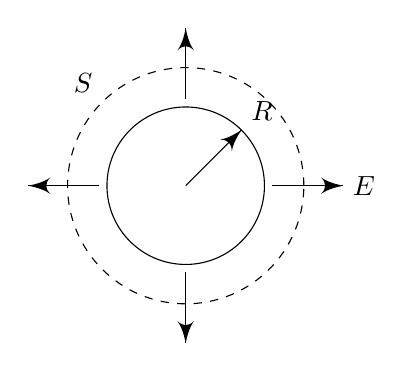
\begin{tikzpicture}
      \draw circle [radius=1];
      \draw [->] (0, 0) -- (.71, .71) node [anchor=south west] {$R$};
      \draw [->] (0, 1.1) -- (0, 2);
      \draw [->] (0, -1.1) -- (0, -2);
      \draw [->] (1.1, 0) -- (2, 0) node [right] {$E$};
      \draw [->] (-1.1, 0) -- (-2, 0);
      \draw [dashed] circle [radius=1.5];
      \node at (-1.06, 1.06) [anchor=south east] {$S$};
    \end{tikzpicture}
  \end{center}

  By symmetry, the force is the same in all directions and point outward radially. So
  \[
    \mathbf{E} = E(r) \hat{\mathbf{r}}.
  \]
  This immediately ensures that $\nabla \times \mathbf{E} = 0$.

  Put $S$ to be a sphere of radius $r > R$. Then
  \begin{align*}
    \int_S \mathbf{E}\cdot \d \mathbf{S} &= \int_S E(r) \hat{\mathbf{r}}\cdot \d \mathbf{S}\\
    &= E(r) \int_S \hat{\mathbf{r}}\cdot \d \mathbf{S}\\
    &= E(r)\cdot 4\pi r^2\\
    &= \frac{Q}{\varepsilon_0}
  \end{align*}
  We were able to pull the $E(r)$ out since it is constant over the sphere.

  Therefore
  \[
    \mathbf{E}(r) = \frac{Q}{4\pi\varepsilon_0 r^2}\hat{\mathbf{r}}.
  \]
  The Lorentz force law tells us that the force experienced by a second charge is
  \[
    \mathbf{F}(\mathbf{r}) = \frac{Qq}{4\pi\varepsilon_0 r^2}\hat{\mathbf{r}},
  \]
  which is Columb's law. Note that strictly speaking, this only holds when the charges are not moving. However, we can still use this because the corrections when they move are tiny.
\end{eg}

\begin{eg}
  Consider a uniform sphere with
  \[
    \rho (r) = \begin{cases}
      \rho & r < R\\
      0 & r > R
    \end{cases}.
  \]
  Outside, we know that 
  \[
    \mathbf{E} = \frac{Q}{4\pi\varepsilon_0 r^2}\hat{\mathbf{r}}
  \]

  Now suppose we are inside the sphere.
   \begin{center}
    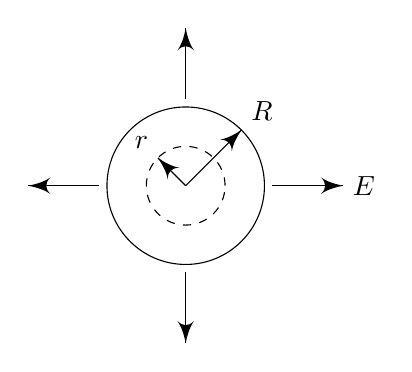
\begin{tikzpicture}
      \draw circle [radius=1];
      \draw [->] (0, 0) -- (.71, .71) node [anchor=south west] {$R$};
      \draw [->] (0, 1.1) -- (0, 2);
      \draw [->] (0, -1.1) -- (0, -2);
      \draw [->] (1.1, 0) -- (2, 0) node [right] {$E$};
      \draw [->] (-1.1, 0) -- (-2, 0);
      \draw [dashed] circle [radius=0.5];
      \draw [->] (0, 0) -- (-.353, .353) node [anchor=south east] {$r$};
    \end{tikzpicture}
  \end{center}

  Then
  \begin{align*}
    \int_S \mathbf{E}\cdot \d\mathbf{S} &= E(r) 4\pi r^2\\
    &= \frac{Q}{\varepsilon_0}\left(\frac{r^3}{R^3}\right)
  \end{align*}
  
  So 
  \[
    \mathbf{E}(r) = \frac{Qr}{4\pi\varepsilon_0 R^3}\hat{\mathbf{r}},
  \]
  and the field increases with radius. 
\end{eg}

\begin{eg}[Line charge]
  Consider an infinite line with uniform charge density \emph{per unit length} $\eta$.

  We use cylindrical polar coordinates:
  \begin{center}
    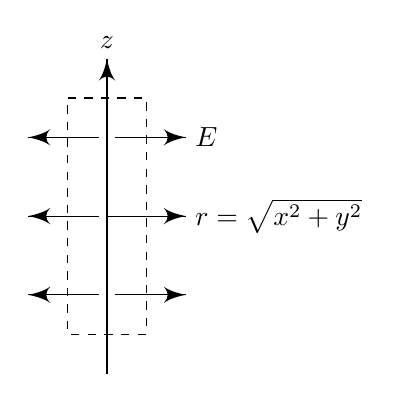
\begin{tikzpicture}
      \draw [->] (0, -2) -- (0, 2) node [above] {$z$};
      \draw [->] (0, 0) -- (1, 0) node [right] {$r = \sqrt{x^2 + y^2}$};

      \draw [->] (0.1, 1) -- (1, 1) node [right] {$E$};
      \draw [->] (-0.1, 1) -- (-1, 1);
      \draw [->] (-0.1, 0) -- (-1, 0);
      \draw [->] (0.1, -1) -- (1, -1);
      \draw [->] (-0.1, -1) -- (-1, -1);

      \draw [dashed] (-0.5, 1.5) -- (0.5, 1.5) -- (0.5, -1.5) -- (-0.5, -1.5) -- cycle;
    \end{tikzpicture}
  \end{center}

  By symmetry, the field is radial, ie.
  \[
    \mathbf{E}(r) = E(r) \hat{\mathbf{r}}.
  \]
  Pick $S$ to be a cylinder of length $L$ and radius $r$. We know that the end caps do not contribute to the flux since the field lines are perpendicular to the normal. Then
  \[
    \int_S\mathbf{E}\cdot \mathbf{S} = E(r)2\pi rL = \frac{\eta L}{\varepsilon_0}.
  \]
  So
  \[
    \mathbf{E}(r) = \frac{\eta}{2\pi \varepsilon_0 r} \hat{\mathbf{r}}.
  \]
  Note that the field varies as $1/r$, not $1/r^2$. Intuitively, this is because we have one more dimension of ``stuff'' compared to the point charge. 
\end{eg}

\begin{eg}[Surface charge]
  Consider an infinite plane $z = 0$, with uniform charge per unit area $\sigma$.

  \begin{center}
    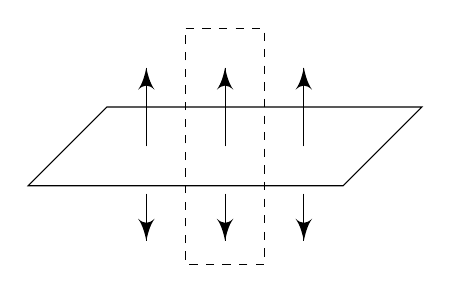
\begin{tikzpicture}
      \draw (-2.5, -.5) -- (1.5, -.5) -- (2.5, .5) -- (-1.5, .5) -- cycle;
      \draw [->] (0, 0) -- (0, 1);
      \draw [->] (-1, 0) -- (-1, 1);
      \draw [->] (1, 0) -- (1, 1);
      
      \draw [->] (0, -.6) -- (0, -1.2);
      \draw [->] (1, -.6) -- (1, -1.2);
      \draw [->] (-1, -.6) -- (-1, -1.2);

      \draw [dashed] (-0.5, 1.5) -- (0.5, 1.5) -- (0.5, -1.5) -- (-0.5, -1.5) -- cycle;
    \end{tikzpicture}
  \end{center}

  By symmetry, the field points vertically, and the field bottom is the opposite of that on top. we must have
  \[
    \mathbf{E} = E(z)\hat{\mathbf{z}}
  \]
  with
  \[
    E(z) = -E(-z).
  \]
  Consider a vertical cylinder of height $2z$ and cross-sectional area $A$. Now only the end caps contribute.
  \begin{align*}
    \int_S \mathbf{E} \cdot \d \mathbf{S} &= E(z) A - E(-z) A\\
    &=\frac{\sigma A}{\varepsilon _0}. 
  \end{align*}
  So
  \[
    E(z) = \frac{\sigma }{2\varepsilon_0}
  \]
  and is constant.

  Note that the electric field is discontinuous across the surface. We have
  \[
    E(z\to 0+) - E(z\to 0-) = \frac{\sigma}{\varepsilon_0}.
  \]
  Note that this is a general result that is true for any arbitrary surfaces and $\sigma$. We can prove this by considering a cylinder across the surface and then shrink it indefinitely. The we find that
  \[
    \hat{\mathbf{n}}\cdot \mathbf{E}_+ - \hat{\mathbf{n}}\cdot \mathbf{E}_- = \frac{\sigma}{\varepsilon_0}.
  \]
  However, the components of $\mathbf{E}$ tangential to the sruface are continuous. 
\end{eg}

\subsection{Electrostatic potential}
In general, we will have to solve both $\nabla \cdot \mathbf{E} = \rho/\varepsilon_0$ and $\nabla \times \mathbf{E} = \mathbf{0}$. However, we already know that the general form of the solution to the second equation is $\mathbf{E} = -\nabla\phi$ for some scalar field $\phi$.
\begin{defi}[Electrostatic potential]
  If $\mathbf{E} = -\nabla \phi$, then $\phi$ is the \emph{electrostatic potential}.
\end{defi}
Then
\[
  \nabla\cdot \mathbf{E} = \frac{\rho}{\varepsilon_0} \Rightarrow \nabla^2\phi = \frac{\rho}{\varepsilon_0},
\]
which is the \emph{Poisson equation}. If we are in the middle of nowhere and $\rho = 0$, then we just get the \emph{Laplace equation}.

Note the following:
\begin{itemize}
  \item $\phi$ is only defined up to a constant. We usually fix this by insisting $\phi(\mathbf{r}) \to 0$ as $r\to \infty$. Note that this statement seems trivial, but this property of $\phi$ is actually very important and gives rise to a lot of interesting properties, as we will see later.
  \item The Poisson equation is linear. So if we have two charges $\rho = \rho_1 + \rho_1$, then $\phi = \phi_1 + \phi_2$ and $\mathbf{E} = \mathbf{E}_i + \mathbf{E}_2$. This is the \emph{principle of superposition}. Among the four fundamental forces of nature, electromagnetism is the only force with this property.
\end{itemize}
\subsubsection{Point charge}
Consider a point particle with charge $Q$ at the origin. Then
\[
  \rho (\mathbf{r}) = Q\delta^3(\mathbf{r}).
\]
The power 3 of the delta function indicates that it is for a 3-dimensional vector.

We have to solve
\[
  \nabla^2\phi = -\frac{Q}{\varepsilon_0}\delta^3(\mathbf{r}).
\]
Away from the origin $\mathbf{r} = \mathbf{0}$, the solution is just
\[
  \phi = \frac{\alpha}{r}\quad \text{for some constant }\alpha
\]
We check this by noting $\nabla r = \mathbf{r}/|r| = \hat{\mathbf{r}}$. So
\[
  \nabla\left(\frac{\alpha}{r}\right)^3 = \frac{-\alpha\mathbf{r}}{r^3}.
\]
and thus
\[
  \nabla^2 \phi = -\alpha\left(\frac{\nabla\cdot \mathbf{r}}{r^2} - 3\frac{\mathbf{r}\cdot \mathbf{r}}{r^5}\right) = 0.
\]
The constant $\alpha$ is determined by the delta function. We integrate over a sphere centered at the origin to obtain
\[
  \int_V \nabla^2\phi\;\d V = \int_S \nabla\phi\cdot\d \mathbf{S} = -\frac{Q}{\varepsilon_0}\int_V\delta^3(r)\; \d V = -\frac{Q}{\varepsilon_0}.
\]
Substitute $\phi = \alpha/r$. $\nabla \phi = -\alpha/r^2$ points in the same direction as $\d \mathbf{S}$, and is integrated over a surface area of $4\pi r^2$. So the surface integral is $-4\pi\alpha$ and $\alpha = Q/(4\pi\varepsilon_0)$. So
\[
  \mathbf{E} = -\nabla \phi = \frac{Q}{4\pi\varepsilon_0 r^2}\hat{\mathbf{r}}.
\]

\subsubsection{Dipole}
\begin{defi}[Dipole]
  A \emph{dipole} consists of two point charges, $+Q$ and $-Q$ at $\mathbf{r} = 0$ and $\mathbf{r} = -\mathbf{d}$ respectively. By the principle of superposition,
  \[
    \phi = \frac{1}{4\pi\varepsilon_0}\left(\frac{Q}{r} - \frac{Q}{|\mathbf{r} + \mathbf{d}|}\right).
  \]
\end{defi}

We can ask what the scalar field looks like at a distance $r \gg d$. We work with the vector version of Taylor expansion:
\[
  f(\mathbf{r} + \mathbf{d}) = f(\mathbf{r}) + \mathbf{d}\cdot \nabla f(\mathbf{r}) + \frac{1}{2}(\mathbf{d}\cdot \nabla)^2f(\mathbf{r}) + \cdots.
\]
So
\begin{align*}
  \frac{1}{|\mathbf{r} + \mathbf{d}} &= \frac{1}{r} - \mathbf{d}\cdot \nabla\left(\frac{1}{r}\right) + \frac{1}{2}(\mathbf{d}\cdot \nabla)^2\left(\frac{1}{r}\right)\\
  &= \frac{1}{r} - \frac{\mathbf{d}\cdot \mathbf{r}}{r^3} - \frac{1}{2}\left(\frac{\mathbf{d}\cdot \mathbf{d}}{r^3} - \frac{3(\mathbf{d}\cdot \mathbf{r})^2}{r^5} + \cdots\right)
\end{align*}
For the dipole we have
\[
  \phi = \frac{Q}{4\pi\varepsilon_0}\left(\frac{1}{r} - \frac{1}{r} + \frac{\mathbf{d}\cdot \mathbf{r}}{r^3} + \cdots\right) \sim \frac{Q}{4\pi\varepsilon_0} \frac{\mathbf{d}\cdot \mathbf{r}}{r^3}.
\]
\begin{defi}[Electric dipole moment]
  We define the \emph{electric dipole moment} is
  \[
    \mathbf{p} = Q\mathbf{d}.
  \]
  By convention, it points from -ve to +ve.
\end{defi}
Then
\[
  \phi = \frac{\mathbf{p}\cdot \hat{\mathbf{r}}}{4\pi\varepsilon_0 r^2},
\]
and
\[
  \mathbf{E} = -\nabla\phi = \frac{1}{4\pi\varepsilon_0}\left(\frac{3(\mathbf{p}\cdot\hat{\mathbf{r}})\hat{\mathbf{r}} - \mathbf{p}}{r^3}\right).
\]
Note that this is \emph{weird}.

\subsubsection{General charge distribution}
To find $\phi$ for a general charge distribution $\rho$, we use the Green's function for the Laplacian
\[
  \nabla^2 G(\mathbf{r}, \mathbf{r}') = \delta^3(\mathbf{r} - \mathbf{r}'),
\]
where
\[
  G(\mathbf{r}, \mathbf{r}') = -\frac{1}{4\pi}\frac{1}{|\mathbf{r} - \mathbf{r}'|}.
\]
We'll take $\rho(\mathbf{r})\not= 0$ only on some compact region $V$. Then
\begin{align*}
  \phi(\mathbf{r}) &= -\frac{1}{\varepsilon_0}\int_V \rho(\mathbf{r}') G(\mathbf{r}, \mathbf{r}')\;\d V\\
  &= \frac{1}{4\pi\varepsilon_0}\int_V \frac{\rho(\mathbf{r}')}{|\mathbf{r} - \mathbf{r}'|}\;\d V
\end{align*}
Note that inside the integral, we are integrating against $\mathbf{r}'$.

This works because if we apply $\nabla^2$ to $\phi(\mathbf{r})$, then $\mathbf{r}'$ terms are unaffected because we are differentiating wrt $\mathbf{r}$, and only $G(\mathbf{r}, \mathbf{r}')$ is differentiated to the delta function $\delta^3(\mathbf{r} - \mathbf{r}')$. Then the integral becomes $\rho(\mathbf{r}')$, which gives $\nabla^2 \phi = \rho/\varepsilon_0$, in accordance with Maxwell's equation.

Then
\begin{align*}
  \mathbf{E}(\mathbf{r}) &= -\nabla \phi(\mathbf{r})\\
  &=- \frac{1}{4\pi\varepsilon_0} \int_V \rho(\mathbf{r})\nabla \left(\frac{1}{|\mathbf{r} - \mathbf{r}'|}\right)\;\d V\\
  &= \frac{1}{4\pi\varepsilon_0}\int_V \rho(\mathbf{r}')\frac{(\mathbf{r} - \mathbf{r}')}{|\mathbf{r} - \mathbf{r}'|^3}\;\d V
\end{align*}
So if we plug in a very complicated $\rho$, we get a very complicated $\mathbf{E}$!

However, we can ask what $\phi$ and $\mathbf{E}$ look like very far from $V$, ie. $|\mathbf{r}| \gg |\mathbf{r}'|$. 

We again use the Taylor expansion.
\begin{align*}
  |\mathbf{r} - \mathbf{r}'| &= \frac{1}{r} + \mathbf{r}'\cdot \nabla\left(\frac{1}{r}\right) + \cdots\\
  &= \frac{1}{r} + \frac{\mathbf{r}\cdot \mathbf{r}'}{r^3} + \cdots
\end{align*}
Then
\begin{align*}
  \phi(\mathbf{r}) &= \frac{1}{4\pi\varepsilon_0} \int_V \rho(\mathbf{r}')\left(\frac{1}{r} + \frac{\mathbf{r}\cdot \mathbf{r}'}{r^3} + \cdots\right)\;\d V\\
  &= \frac{1}{4\pi\varepsilon_0}\left(\frac{Q}{r} + \frac{\mathbf{p}\cdot \hat{\mathbf{r}}}{r^2} + \cdots\right)
\end{align*}
Where
\begin{align*}
  Q &= \int_V \rho(\mathbf{r}')\;\d V \\
  \mathbf{p} &= \int_V \mathbf{r}'\rho(\mathbf{r}')\; \d V
\end{align*}
So if we have a huge lump of charge, we can consider it to be a point charge $Q$, plus some dipole correction terms. 
\subsubsection{Field lines and equipotentials}
\begin{defi}[Field line]
  A \emph{field line} is a continuous line tangent to the electric field $\mathbf{E}$. The density of lines is proportional to $|\mathbf{E}|$ The begin and end only at charges (and infinity). They never cross.
\end{defi}

\begin{defi}[Equipotentials]
  \emph{Equipotentials} are surfaces of constant $\phi$. Because $\mathbf{E} = -\nabla \phi$, they are always perpendicular to field lines.
\end{defi}
\begin{eg}\leavevmode
  \begin{center}
    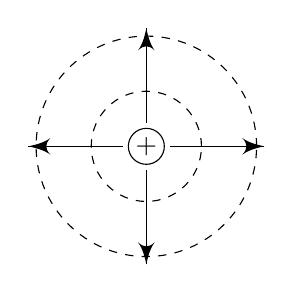
\begin{tikzpicture}
      \node [draw, circle, inner sep = 0, minimum size=13] {+};
      \draw [dashed] circle [radius=1.4];
      \draw [dashed] circle [radius=.7];
      \draw [->] (0, 0.3) -- (0, 1.5);
      \draw [->] (0.3, 0) -- (1.5, 0);
      \draw [->] (0, -0.3) -- (0, -1.5);
      \draw [->] (-0.3, 0) -- (-1.5, 0);
    \end{tikzpicture}
    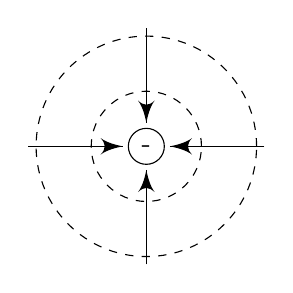
\begin{tikzpicture}
      \node [draw, circle, inner sep = 0, minimum size=13] {-};
      \draw [dashed] circle [radius=1.4];
      \draw [dashed] circle [radius=.7];
      \draw [->] (0, 1.5) -- (0, 0.3);
      \draw [->] (1.5, 0) -- (0.3, 0);
      \draw [->] (0, -1.5) -- (0, -0.3);
      \draw [->] (-1.5, 0) -- (-0.3, 0);
    \end{tikzpicture}
  \end{center}
  Use your imagination to join the two diagrams together to get the field lines for dipoles.
\end{eg}

\subsection{Electrostatic energy}
We want to calculate how much energy is stored in the electric field. Recall from Dynamics and Relativity that a particle of charge $q$ in a field $\mathbf{E} = -\nabla \phi$ has potential energy $U(\mathbf{r}) = q\phi(\mathbf{r})$.

$U(\mathbf{r})$ can be thought of as the work done in bringing the particle from infinity, as illustrated below:
\begin{align*}
  \text{work done} &= -\int_\infty^\mathbf{r} \mathbf{F}\cdot \d \mathbf{r}\\
  &= -\int_\infty^\mathbf{r}\mathbf{E}\cdot \d \mathbf{r} \\
  &= q\int_\infty^\mathbf{r} \nabla \mathbf{\phi}\cdot \d \mathbf{r}\\
  &= q[\phi(\mathbf{r}) - \phi(\infty)]\\
  &= U(\mathbf{r})
\end{align*}
where we set $\phi(\infty) = 0$.

Now consider $N$ charges $q_i$ at positions $\mathbf{r}_i$. The total potential energy stored is the work done to assemble these particles. Let's put them in one by one.
\begin{enumerate}
  \item The first charge is free. The work done is $W_1 = 0$.
  \item To place the second charge at position $\mathbf{r}_2$ takes work. The work is
    \[
      W_2 = \frac{q_1q_1}{4\pi\varepsilon_0}\frac{1}{|\mathbf{r}_1 - \mathbf{r}_2|}.
    \]
  \item To place the third charge at position $\mathbf{r}_3$, we do
    \[
      W_3 = \frac{q_3}{4\pi\varepsilon_0}\left(\frac{q_1}{|\mathbf{r}_1 - \mathbf{r}_3|} - \frac{q_2}{|\mathbf{r}_2 - \mathbf{r}_3|}\right)
    \]
  \item etc.
\end{enumerate}
The total work done is
\begin{prop}
  \[
    U = \sum_{i = 1}^N W_i = \frac{1}{4\pi\varepsilon_0} \sum_{i < j} \frac{q_iq_j}{|\mathbf{r}_i - \mathbf{r}_j|}.
  \]
  Equivalently, 
  \[
    U = \frac{1}{4\pi\varepsilon_0} \frac{1}{2} \sum_{i \not= j} \frac{q_1q_1}{|\mathbf{r}_i - \mathbf{r}_j|}.
  \]
  Now the potential at point $\mathbf{r}_i$ due to all $q_j$ with $j\not= i$ is
  \[
    \phi(\mathbf{r}_i) = \frac{1}{4\pi\varepsilon_0}\sum_{j\not= i}\frac{q}{|\mathbf{r}_i - \mathbf{r}_j|}.
  \]
  So
  \[
    U = \frac{1}{2}\sum_{i = 1}^N q_i \phi(\mathbf{r}_i).
  \]
\end{prop}
There is an obvious generalization to continuous charge distributions:
\begin{prop}
  \[
    U = \frac{1}{2} \int \rho (\mathbf{r}) \phi(\mathbf{r}) \;\d V.
  \]
\end{prop}
\note There is a subtlety here, and there is an extra contribution to the work done in this integral. cf. official notes.

Now we can write
\begin{prop}
  \begin{align*}
    U &= \frac{\varepsilon_0}{2}\int (\nabla\cdot \mathbf{E}) \phi \;\d V\\
    &= \frac{\varepsilon_0}{2}\int [\nabla\cdot (\mathbf{E}\phi) - \mathbf{E}\cdot \nabla \phi]\;\d V\\
    &= \frac{\varepsilon_0}{2}\int \mathbf{E}\cdot \mathbf{E} \;\d V.
  \end{align*}
\end{prop}

\subsection{Conductors}
\begin{defi}[Conductor]
  A \emph{conductor} is a region of space which contains lots of charges that are free to move.
\end{defi}
\note
\begin{itemize}
  \item In electrostatic situations, we must have $\mathbf{E} = 0$ inside a conductor. Otherwise, the charges inside the conductor would move till equilibrium. This almost describes the whole of the section: if you apply an electric field onto a conductor, the charges inside the conductor move until the external field is canceled out.
  \item Since $\mathbf{E} = 0$, $\phi$ is constant inside the conductor.
  \item Since $\nabla \cdot \mathbf{E} = \varepsilon/\varepsilon_0$, $\rho = 0$ inside a conductor, ie. the charges must cancel out inside. So any net charge has to live on the surface.
  \item $\mathbf{E} = -\nabla \phi$ is true, and $\phi$ constant in conductor means $\mathbf{E}$ is perpendicular to the surface.
  \item If there is some surface charge $\sigma$, then the discontinuity of $\mathbf{E}$ gives us $\mathbf{E}_\text{outside} = \frac{\sigma}{\varepsilon_0} \hat{\mathbf{n}}$.
\end{itemize}

There are two typical kinds of problems.
\begin{enumerate}
  \item The total charge $Q$ on a conductor is fixed. 
    \begin{eg}
      Consider a spherical conductor with $Q = 0$ in a constant electric field $\mathbf{E}$. Since the electric field lines must be perpendicular to the surface, they have to bend towards the conductor. Since field lines end and start at charges, there must be negative charges at the left and positive charges at the right.
      \begin{center}
        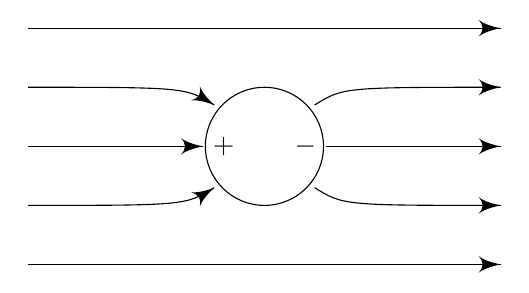
\begin{tikzpicture}
          \draw circle [radius=.75];
          \draw [->] (-3, 1.5) -- (3, 1.5);
          \draw [->] (-3, -1.5) -- (3, -1.5);
          \draw [->] (-3, 0.75) .. controls (-1, 0.75) .. (-.6375, .525);
          \draw [->] (.6375, .525) .. controls (1, 0.75) .. (3, 0.75);
          \draw [->] (-3, -0.75) .. controls (-1, -0.75) .. (-.6375, -.525);
          \draw [->] (.6375, -.525) .. controls (1, -0.75) .. (3, -0.75);
          \draw [->] (-3, 0) -- (-.78, 0) node [right] {$+$};
          \draw [->] (.78, 0) node [left] {$-$} -- (3, 0);
        \end{tikzpicture}
      \end{center}
      We get an induced surface charge and we want to figure out both $\mathbf{E}$ and $\sigma$.
    \end{eg}
  \item The conductor is of fixed potential $\phi$, usually taken to be $\phi = 0$. The conductor is said to be \emph{grounded}, i.e. attached to the Earth.

    \note In the first case, the potential is constant in any particular environment, but can change when the environment changes. In this case, the potential is always 0 regardless of what the world looks like.

    \begin{eg}\leavevmode
      \begin{center}
        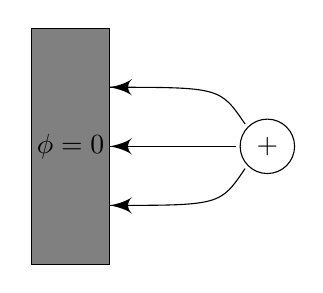
\begin{tikzpicture}
          \draw [fill=gray] (-1, 1.5) rectangle (0, -1.5);
          \node at (-0.5, 0) {$\phi = 0$};
          \node [draw, circle] at (2, 0) {$+$};
          \draw [->] (1.6, 0) -- (0, 0);
          \draw [->] (1.7172, .2828) .. controls (1.4, 0.75) .. (0, 0.75);
          \draw [->] (1.7172, -.2828) .. controls (1.4, -0.75) .. (0, -0.75);
        \end{tikzpicture}
      \end{center}

      Suppose we have a conductor that fills all space $x < 0$. We ground it so that $\phi = 0$ through the plane. Then we place a charge $q$ at $x = d > 0$.

      We are looking for a solution with a source at $x = d$ and $\phi = 0$ at $x = 0$. We know that there is a unique solution.

      We use the method of images, and pretend that instead of a conductor, we have a charge $-q$ at $x = -d$. The potential for this pair is just
      \[
        \phi = \frac{1}{4\pi\varepsilon_0}\left[\frac{q}{\sqrt{(x - d)^2 + y^2 + z^2}} - \frac{q}{\sqrt{(x + d)^2 + y^2 + z^2}}\right].
      \]
      This has $\phi = 0$ at $x = 0$, with a point source at $x = d$. Since this solves our original equation, it must by THE solution.

      We can compute
      \[
        \mathbf{E}_x = -\frac{\partial \phi}{\partial x} = \frac{q}{4\pi\varepsilon_0}\left(\frac{x - d}{|\mathbf{r} - \mathbf{d}|^{3/2}} - \frac{x + d}{|\mathbf{r} + \mathbf{d}|^{3/2}}\right)
      \]
      for $x > 0$. The induced surface charge is
      \[
        \sigma = E_x\varepsilon_0|_{x = 0^+} = -\frac{q}{2\pi}\frac{d}{(d^2 + y^2 + z^2)^{3/2}}.
      \]
      The surface charge is 
      \[
        q = \int \sigma \;\d y\;\d z  = -q.
      \]
    \end{eg}
\end{enumerate}
\section{Magnetostatics}
Charges always give rise to electric fields. Currents give rise to magnetic fields. We will look for time independent solutions to the Maxwell's equation with $\mathbf{J}\not= 0$ and $\rho = 0$. We need to solve
\begin{align*}
  \nabla \times \mathbf{B} &= \mu \mathbf{J}\\
  \nabla\cdot \mathbf{B} &= 0
\end{align*}
The goal is, given $\mathbf{J}$, find $\mathbf{B}$.

\note $\rho = 0$ and $\mathbf{J} \not= 0$ means that we have equal positive and negative charges that can move.

Recall the conservation of charge:
\[
  \frac{\partial\rho}{\partial t} + \nabla \cdot \mathbf{J} = 0.
\]
In this case, since $\rho = 0$, we must have
\[
  \nabla\cdot \mathbf{J} = 0.
\]
These are \emph{steady currents}.
\subsection{Ampere's Law}
Consider a surface $S$ with boundary $C$. Current $\mathbf{J}$ flows through $S$. We now integrate the first equation over the surface $S$ to obtain
\[
  \int_S (\nabla\times \mathbf{B})\cdot \d S = \oint_C \mathbf{B}\cdot \d \mathbf{r} = \mu_0 \int_S \mathbf{J}\cdot \d S.
\]
So
\begin{law}[Ampere's law]
  \[
    \oint_C \mathbf{B}\cdot \d \mathbf{r} = \mu I,
  \]
  where $I$ is the current through the surface.
\end{law}

\begin{eg}[A long straight wire]
  A wire is a cylinder with current $I$ flowing through it.

  We use cylindrical polar coordinates $(r, \varphi, z)$, where $z$ is along the direction of the current, and $r$ points in the radial direction.

  \begin{center}
    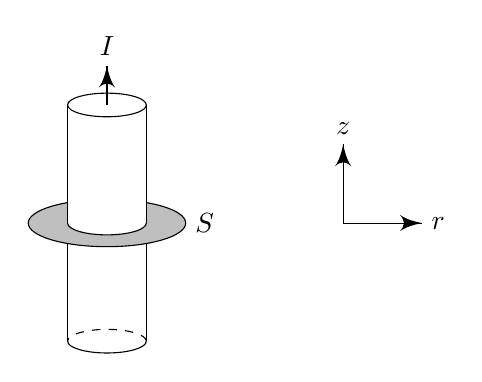
\begin{tikzpicture}
      \draw (0, 1.5) circle [x radius=0.5, y radius = 0.15];
      \draw [dashed] (0.5, -1.5) arc (0: 180:0.5 and 0.15);
      \draw (-0.5, -1.5) arc (180: 360:0.5 and 0.15);
      \draw (0.5, 1.5) -- (0.5, -1.5);
      \draw (-0.5, 1.5) -- (-0.5, -1.5);

      \draw [->] (0, 1.5) -- (0, 2) node [above] {$I$};

      \draw [fill = gray!50!white] circle [x radius = 1, y radius = 0.3];
      \draw [fill = white] circle [x radius = 0.5, y radius = 0.15];
      \draw [fill = white, draw = none] (-0.5, 0) rectangle (0.5, 1);
      \draw (-0.5, 0) -- (-0.5, 1);
      \draw (0.5, 0) -- (0.5, 1);
      \node at (1, 0) [right] {$S$};

      \draw [->] (3, 0) -- (3, 1) node [above] {$z$};
      \draw [->] (3, 0) -- (4, 0) node [right] {$r$};
    \end{tikzpicture}
  \end{center}

  We integrate over a disc that cuts through the wire horizontally.

  We need $\oint_C \mathbf{B}\cdot d\mathbf{r} = \mu_o I$. By symmetry, we have
  \[
    \mathbf{B}(\mathbf{r}) = B(r)\hat{\varphi}.
  \]
  This automatically satisfies $\nabla \cdot \mathbf{B} = 0$.
  Then
  \[
    \oint_C \mathbf{B}\cdot \d \mathbf{r}  =B(r)\int_0^{2\pi} r\;\d \varphi = 2\pi rB(r) = \mu_0 I.
  \]
  So
  \[
    \mathbf{B}(r) = \frac{\mu_0 I}{2\pi r} \hat{\varphi}.
  \]
\end{eg}

\begin{eg}[Surface current]
  Consider the plane $z = 0$ with \emph{surface current density} $\mathbf{k}$ (i.e. current per unit length).
  \begin{center}
     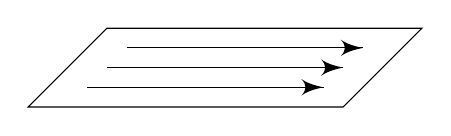
\begin{tikzpicture}[
        y  = {(0.5cm,0.5cm)},
        z  = {(0cm,1cm)}]
      \draw (-2, -1, 0) -- (2, -1, 0) -- (2, 1, 0) -- (-2, 1, 0) -- cycle;
      \draw [->] (-1.5, 0.5, 0) -- (1.5, 0.5, 0);
      \draw [->] (-1.5, -0.5, 0) -- (1.5, -0.5, 0);
      \draw [->] (-1.5, 0, 0) -- (1.5, 0, 0);
    \end{tikzpicture}
  \end{center}

  Take the x-direction to be the direction of the current, and the z direction to be the normal to the plane.

  We imagine this situation by considering to be infinitely many copies of the above wire situation. Then the magnetic fields must point in the y-direction. By symmetry, we must have
  \[
    \mathbf{B} = -B(z) \hat{\mathbf{y}},
  \]
  with $B(z) = -B(-z)$.

  Consider a vertical rectangular loop of length $L$ through the surface
  \begin{center}
    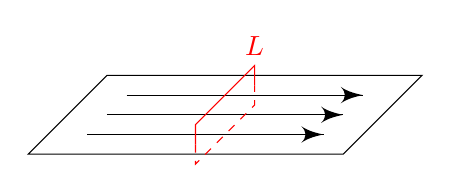
\begin{tikzpicture}[
        y  = {(0.5cm,0.5cm)},
        z  = {(0cm,1cm)}]
      \draw (-2, -1, 0) -- (2, -1, 0) -- (2, 1, 0) -- (-2, 1, 0) -- cycle;
      \draw [->] (-1.5, 0.5, 0) -- (1.5, 0.5, 0);
      \draw [->] (-1.5, -0.5, 0) -- (1.5, -0.5, 0);
      \draw [->] (-1.5, 0, 0) -- (1.5, 0, 0);
      \draw [red] (0, 0.75, 0) -- (0, 0.75, 0.25) node [above] {$L$} -- (0, -0.75, 0.25) -- (0, -0.75, 0);
      \draw [dashed, red] (0, -0.75, 0) -- (0, -0.75, -0.25) -- (0, 0.75, -0.25) -- (0, 0.75, 0);
    \end{tikzpicture}
  \end{center}
  Then
  \[
    \oint_C \mathbf{B}\cdot \d \mathbf{r} = LB(z) - LB(-z) = \mu_0 kL
  \]
  So
  \[
    B(z) = \frac{\mu_0 k}{2}\quad\text{ for }z > 0.
  \]
  Similar to the electrostatic case, the magnetic field is constant, and the part parallel to the surface is discontinuous across the plane. This is a general result, ie. across any surface,
  \[
    \hat {\mathbf{n}} \times \mathbf{B}_+ - \hat{\mathbf{n}}\times \mathbf{B}_{-} = \mu_0 \mathbf{k}.
  \]
\end{eg}

\begin{eg}[Solenoid]
  A \emph{solenoid} is a cylindrical surface current, usually made by wrapping a wire around a cylinder.
  \begin{center}
    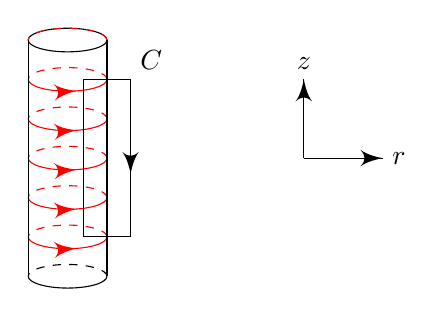
\begin{tikzpicture}
      \draw (0, 1.5) circle [x radius=0.5, y radius = 0.15];
      \draw [dashed] (0.5, -1.5) arc (0: 180:0.5 and 0.15);
      \draw (-0.5, -1.5) arc (180: 360:0.5 and 0.15);
      \draw [red, dashed] (0.5, -1) arc (0: 180:0.5 and 0.15); %insert arrows
      \draw [red, ->-=0.6] (-0.5, -1) arc (180: 360:0.5 and 0.15);
      \draw [red, dashed] (0.5, -0.5) arc (0: 180:0.5 and 0.15);
      \draw [red, ->-=0.6] (-0.5, -0.5) arc (180: 360:0.5 and 0.15);
      \draw [red, dashed] (0.5, 0) arc (0: 180:0.5 and 0.15);
      \draw [red, ->-=0.6] (-0.5, 0) arc (180: 360:0.5 and 0.15);
      \draw [red, dashed] (0.5, 0.5) arc (0: 180:0.5 and 0.15);
      \draw [red, ->-=0.6] (-0.5, 0.5) arc (180: 360:0.5 and 0.15);
      \draw [red, dashed] (0.5, 1) arc (0: 180:0.5 and 0.15);
      \draw [red, ->-=0.6] (-0.5, 1) arc (180: 360:0.5 and 0.15);
      \draw [red, dashed] (0.5, 1.5) arc (0: 180:0.5 and 0.15);
      \draw (0.5, 1.5) -- (0.5, -1.5);
      \draw (-0.5, 1.5) -- (-0.5, -1.5);

      \draw [->] (3, 0) -- (3, 1) node [above] {$z$};
      \draw [->] (3, 0) -- (4, 0) node [right] {$r$};

      \draw (0.2, 1) -- (0.8, 1) node[anchor = south west] {$C$};
      \draw [->-=0.6] (0.8, 1) -- (0.8, -1);
      \draw (0.8, -1) -- (0.2, -1) -- (0.2, 1);
    \end{tikzpicture}
  \end{center}


  We use cylindrical polar coordinates with $z$ in the direction of the extension of the cylinder. By symmetry, $\mathbf{B} = B(r)\mathbf{z}$.

  Away from the cylinder, $\nabla \times \mathbf{B} = 0$. So $\frac{\partial B}{\partial r} = 0$, which means that $B(r)$ is constant outside. Since we know that $\mathbf{B} = \mathbf{0}$ at infinity, $\mathbf{B} = \mathbf{0}$ everywhere outside the cylinder. 

  To compute $\mathbf{B}$ inside, use Ampere's law with a curve $C$. Note that only the vertical part (say of length $L$) inside the cylinder contributes to the integral. Then
  \[
    \oint_C \mathbf{B}\cdot \d \mathbf{r} = BL = \mu_o INL.
  \]
  where $N$ is the number of wires per unit length and $I$ is the current in each wire (so $INL$ is the total amount of current through the wires).

  So $B = \mu_0 IN$.
\end{eg}

\subsection{Vector potential}
For general current distributions $\mathbf{J}$, we also need to solve $\nabla \cdot \mathbf{B} = 0$.

This is telling us that there are no magnetic monopoles, ie. magnetic charges (cf. electric version, with $\rho = 0$)

We can solve this by writing $\mathbf{B} = \nabla \times \mathbf{A}$.
\begin{defi}[Vector potential]
  If $\mathbf{B} = \nabla\times \mathbf{A}$, then $\mathbf{A}$ is the \emph{vector potential}.
\end{defi}
The other Maxwell equation then says
\[
  \nabla \cdot \mathbf{B} = -\nabla^2 \mathbf{A} + \nabla(\nabla\cdot A) = \mu_0 \mathbf{J}.\tag{$*$}
\]

This is rather difficult to solve, but it can be made easier by noting that:
\begin{prop}[Gauge invariance]
  $\mathbf{A}$ is not unique. If $\mathbf{A}$ is a vector potential, then if 
  \[
    \mathbf{A}' = \mathbf{A} + \nabla \chi
  \]
  for any $\chi(\mathbf{x})$, then $\mathbf{B} = \nabla \times \mathbf{A} = \nabla\times \mathbf{A}'$.

  The transformation $\mathbf{A}' \mapsto \mathbf{A} + \nabla\chi$ is called a\emph{gauge transformation}.
\end{prop}

\begin{defi}[(Coulomb) gauge]
  Each $\mathbf{A}$ is called a \emph{gauge}. An $\mathbf{A}$ such that $\nabla \cdot \mathbf{A} = 0$ is called a \emph{Coulomb gauge}.
\end{defi}
\begin{prop}
  We can always pick $\chi$ such that $\nabla \cdot \mathbf{A}' = 0$.
\end{prop}

\begin{proof}
  Suppose that $\mathbf{B} = \nabla \times \mathbf{A}$ with $\nabla \mathbf{A} = \psi(\mathbf{x})$. Then pick $\mathbf{A}' = \mathbf{A} + \nabla \chi$. Then we have
  \[
    \nabla \cdot \mathbf{A}' = \nabla \mathbf{A} + \nabla^2 \chi = \psi + \nabla^2\chi.
  \]
  Pick $\chi$ such that $\nabla^2\chi = -\psi$. This is the Poisson equation and there is always a solution.
\end{proof}

If $\mathbf{B} = \nabla\times \mathbf{A}$ and $\nabla\cdot \mathbf{A} = 0$, then the Maxwell equation  $(*)$ is
\[
  \nabla^2 \mathbf{A} = -\mu_0 \mathbf{J}.
\]

Or, in Cartesian components,
\[
  \nabla^2 A_i = -\mu_0 J_i.
\]
This is 3 copies of the Poisson equation, which we know how to solve using Green's functions. The solution is
\[
  A_i (\mathbf{r}) = \frac{\mu_0}{4\pi}\int \frac{J_i (\mathbf{r}')}{|\mathbf{r} - \mathbf{r}'|}\;\d V,
\]
or
\[
  \mathbf{A}(\mathbf{r}) = \frac{\mu_0}{4\pi}\int \frac{\mathbf{J}(\mathbf{r'})}{|\mathbf{r} - \mathbf{r}'|}\;\d V,
\]
both integrating over $\mathbf{r}'$.

We have to check \emph{Coulomb gauge}:
\begin{align*}
  \nabla\cdot \mathbf{A}(\mathbf{r}) &= \frac{\mu_0}{4\pi}\int \mathbf{J}(\mathbf{r}')\cdot \nabla\left(\frac{1}{|\mathbf{r} - \mathbf{r}'|}\right)\;\d V\\
  &= -\frac{\mu_0}{4\pi}\int \mathbf{J}(\mathbf{r}') \cdot \nabla'\left(\frac{1}{|\mathbf{r} - \mathbf{r}'|}\right)\;\d V\\
  \intertext{We integrate by parts to obtain}
  &= -\frac{\mu_0}{4\pi}\int \left[\nabla'\cdot \left(\frac{\mathbf{J}(\mathbf{r}')}{|\mathbf{r} - \mathbf{r}'|}\right) - \frac{\nabla' \mathbf{J}(\mathbf{r}')}{|\mathbf{r} - \mathbf{r}'|}\right]\;\d V.
\end{align*}
where $\nabla'$ acts on $\mathbf{r}'$. On the last line, the first term vanishes because we have localized current, while the second vanishes because $\nabla \mathbf{F} = 0$. So $\nabla\cdot \mathbf{A} = 0$.

\begin{law}[Biot-Savart law]
  The magnetic field is
  \[
    \mathbf{B}(\mathbf{r}) = \nabla \times \mathbf{A} = \frac{\mu_0}{4\pi}\int \mathbf{J}(\mathbf{r}')\times \frac{\mathbf{r} - \mathbf{r}'}{|\mathbf{r} - \mathbf{r}'|^3}\;\d V.
  \]
  If the current is localized on a curve, this becomes
  \[
    \mathbf{B} = \frac{\mu_0 I}{4\pi}\oint_C \frac{(\mathbf{r} - \mathbf{r}')}{|\mathbf{r} - \mathbf{r}'|^3}\times \d \mathbf{r}'.
  \]
\end{law}

\subsection{Magnetic dipoles}
We want to ask what $\mathbf{B}$ looks like far from a localized current distribution.

\begin{eg}[Current loop]
  Take a current loop of wire $C$, radius $R$ and current $I$. 
  \begin{center}
    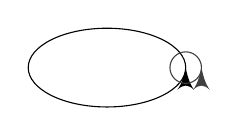
\begin{tikzpicture}
      \draw [->] circle [x radius = 1, y radius = 0.5];
      \draw [->, gray!50!black] (1, 0) circle [radius=0.2];
    \end{tikzpicture}<++>
  \end{center}<++>
  We can guess that $\mathbf{B}$ looks like this, but we want to calculate it.
\end{eg}<++>
\end{document}
